\documentclass{sig-alternate}

\usepackage{amssymb}
\setcounter{tocdepth}{3}
\usepackage{graphicx}
\usepackage{url}

\usepackage{amsmath}
\usepackage{amssymb}
\usepackage{amsfonts}
\usepackage{float}
\usepackage{graphics}
\usepackage{theorem}
\usepackage{euscript}
\usepackage{psfrag}

% MATH -------------------------------------------------------------------
\newcommand{\Real}{\mathcal Re}
\newcommand{\Imaginary}{\mathcal Im}
\newcommand{\RPlus}{\Real^{+}}
\newcommand{\norm}[1]{\left\Vert#1\right\Vert}
\newcommand{\abs}[1]{\left\vert#1\right\vert}
\newcommand{\set}[1]{\left\{#1\right\}}
\newcommand{\seq}[1]{\left<#1\right>}
\newcommand{\eps}{\varepsilon}
\newcommand{\To}{\longrightarrow}
\newcommand{\BX}{\mathbf{B}(X)}
\newcommand{\A}{\mathcal{A}}
\newcommand{\M}{\mathcal{M}}
\newcommand{\N}{\mathcal{N}}
\newcommand{\Lom}{\mathcal{L}}
\newcommand{\Comp}{\mathcal{K}}
\newcommand{\Basis}{\mathcal{B}}

\newcommand{\Bepsilon}{\boldsymbol{\epsilon}}
\newcommand{\Bb}{\text{\textbf{\textit{b}}}}
\newcommand{\Boldit}[1]{\textbf{\textit{#1}}}
\newcommand{\Boldsf}[1]{\textbf{\textsf{#1}}}
\newcommand{\Boldcal}[1]{\mathbf{\mathcal{#1}}}
\newcommand{\Bs}[1]{\boldsymbol{#1}}
\newcommand{\EuS}[1]{\EuScript{#1}}
\newcommand{\Mfr}[1]{\mathfrak{#1}}
\newcommand{\vct}[1]{\boldsymbol{#1}}
\newcommand{\Mat}[1]{\boldsymbol{#1}}

\newtheorem{thm}{Theorem}
\newtheorem{cor}[thm]{Corollary}
\newtheorem{lem}[thm]{Lemma}
\newtheorem{prop}[thm]{Proposition}
\newtheorem{defn}{Definition}
\newtheorem{rem}[thm]{Remark}
\newtheorem{conj}{Conjecture}

\def\E{{\mathbb E}}        % expectation

\def\myscale{0.65}
\def\myhspace{-1.0cm}

\newcommand{\comment}[1]{}
\newcommand{\paren}[1]{\left( #1 \right)}
\newcommand{\bracket}[1]{\left[ #1 \right]}

\newcommand{\argmin}{\operatornamewithlimits{argmin}} 
\newcommand{\argmax}{\operatornamewithlimits{argmax}} 

\newcommand{\remove}[1]{}

\newcommand{\opt}{\ensuremath{i^*}}
\newcommand{\pr}[1]{\ensuremath{\mathbb{P}{(#1)}}}
\newcommand{\meant}[2]{\ensuremath{\hat{X}_{#1,#2}}}
\newcommand{\meanp}[3]{\ensuremath{\hat{X}_{#1,#2}^{#3}}}
\newcommand{\mean}[1]{\ensuremath{\mu_{#1}}}
\newcommand{\delmean}[1]{\ensuremath{\Delta_{#1}}}

\newcommand{\eshcar}[1]{(((Eshcar: #1)))}

\usepackage{etoolbox} \makeatletter \patchcmd{\maketitle}{\@copyrightspace}{}{}{} \makeatother 

\begin{document}

\conferenceinfo{???}{???}
\CopyrightYear{2011}

%\title{The Impact of Index-Partitioning on the Inverted-Index Compression Achieved by Certain Document Reordering Schemes}

%\title{The Impact of Index-Partitioning on the Compression Effectiveness of Document Reordering Schemes}

\title{Multi-Armed Bandit Problem with Distributed Players}

%\author{Anonymous}

\maketitle

%\input{abstract}

%\section{Introduction}


%\input{background}

%\input{setup}

%\input{results}

%\input{discussion}

%\input{concluding}

\begin{abstract}

TBD

\end{abstract}

\section{Introduction}
\begin{itemize}
\item Yahoo!'s front page \textit{Today} module is powered by \textit{explore-exploit multi-armed bandit technology}. To handle the huge traffic load, Yahoo! operates several Colos (or data-centers) distributed accros the US ((depicted in Figure \ref{fig: colos}))
\item Consider a setup where a group of Colos are coomunicating to perform joint explore-exploite Web experiments over a set of users, to determine a certain best outcome (e.g., optimal Web page layout). 
\item There is a range of strategies for sharing data over a broadcast network. The two extremes are (a) no communication - each Colo conducts separate experiments; and (b) full communication - every user interaction is shared to all Colos
\item Reducing the distributed explore-exploit Web experiments setup to a multi-armed bandit framework is done here, by replacing stories/articles, user page views, user clicks, and colos, with arms, arms pulls, rewards, and players, respectively.
\item The idea of multi-armed bandit (MAB) with distributed players was already considered in \cite{Liu-Zhao_IEEE-TSP2010}. However, in that setup the players were not exchanging any information, and a simultaneous arm pull by two or more agents resulted in a collision which was translated to a reward loss or some arbitrary reward sharing between the colliding arms.
\end{itemize}
\comment{
\begin{itemize}
\item Arms $\Longleftrightarrow$ stories/article
\item Arm pulls $\Longleftrightarrow$ user page views
\item Rewards $\Longleftrightarrow$ users' clicks
\item Players $\Longleftrightarrow$ colos
\end{itemize}}

\section{Problem Setup}

\begin{figure}[t]
\centering
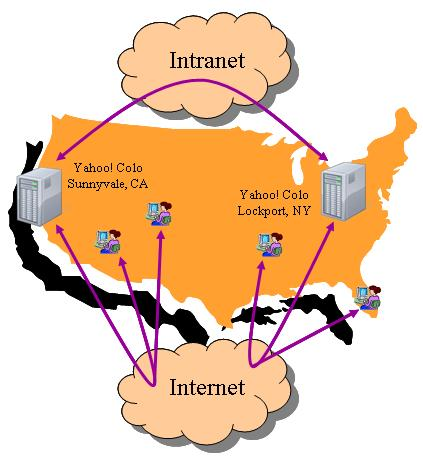
\includegraphics[scale=0.75]{figures/US_Colos.jpg}
\caption{A group of Colos are communicating via Intranet to perform joint MAB/Explore-Exploit experiments over the Internet.}
\label{fig: colos}
\end{figure}

A stochastic multi armed bandit game with distributed players is characterized by the number of arms $K$, total budget of $n$ pulls, and $K$ probability distributions $\nu_1,\ldots,\nu_K$. In contrast to the conventional setup where only one player (forecaster) is involved, here, $M$ players are participating in the game. The players are assumed to be homogeneous in the sense that they have the same utility distribution over the arms. For $t=1,\ldots,n$ rounds, one of the player (determined by round-robin scheduling) selects an arm $I_t$ in the set of arms $\set{1,\ldots,K}$ and observes a reward drawn from $\nu_{I_t}$ independently from past events (actions and observations). We further assume that the players are sharing their information via a delayless and error free backhaul network where a unit cost is charged for every broadcast. 

At the end of the $n$ rounds, the players should unanimously select an arm, denoted $J_n$, which is evaluated in terms of the difference between the mean reword of the optimal arm and the mean reward of $J_n$. In particular, let $\mu_1,\ldots,\mu_K$ be the respective means of $\nu_1,\ldots,\nu_K$. Let $\mu^*=\max_{k\in\set{1,\ldots,K}}\mu_k$. The regret of the decision is $r_n\triangleq\mu^*-\mu_{J_n}$. We also assume binary rewards $\bracket{0,1}$, and that there is a unique optimal arm denoted by $k^*$ (i.e., $\mu_{k^*}=\mu^*$). For arm $k\neq k^*$ we define the gap $\Delta_k=\mu^*-\mu_k$, and the minimum gap $\Delta^*=\min_{\underset{k\neq k^*}{k=1,\ldots,K}}\Delta_k$. We use the notation $\paren{k}$ to denote the $k$th best arm (with random tie break), hence, $\Delta^*=\Delta_{\paren{1}}\le\Delta_{\paren{2}}\le\Delta_{\paren{K}}$. Following \cite{Audibert-Bubeck-Munos-COLT2010} we denote by $e_n$ the error probability $e_n=Pr \paren{J_n\neq i^*}$ and use it as our merit throughout this work since it behaves similarly to the average regret $\E\paren{r_n}$.


For each arm $i$ and all time $t\ge 1$, we denote by $T^m_i(t)$ the number of times arm $i$ was pulled from round $1$ to $t$ by player $m$, and by $X^m_{i,1},\ldots,X^m_{i,T^m_i(t)}$ the sequence of associated rewards. The average reward of arm $i$ at player $m$ after $s$ pulls is denoted $\hat{X}^m_{i,s}\triangleq\frac{1}{s}\sum_{j=1}^s X^m_{i,j}$ while the total average reward of arm $i$ after $s$ pulls is denoted by $\hat{X}_{i,s}\triangleq\frac{1}{M}\sum_{m=1}^M \hat{X}^m_{i,s}$.
\eshcar{These definitions are valid only for algorithms in which different players execute the same number of pulls for a given arm.}

\section{Background and Previous Results}

\subsection{Successive Elimination Algorithm}\label{sec: SE algo}

Successive Elimination Algorithm:
\begin{itemize}
\item Let $A_1=\set{1,\ldots,K}$, $n_0=0$, $n_k\triangleq\lceil \frac{1}{\overline{\log K}}\frac{n-K}{K+1-k}\rceil$ for $k=1,\ldots,K-1$ where $\overline{\log K}\triangleq \frac{1}{2}+\sum_{i=2}^K\frac{1}{i}$ 
\item For each phase $k=1,\ldots,K-1$ do the following:
\begin{itemize}
\item Pull each surviving arm $i\in A_k$, $n_k-n_{k-1}$ times
\item Eliminate the ``worst'' arm (with random tie brakes) $A_{k+1}=A_k\backslash\argmin_{i\in A_k}\set{\hat{X}_{i,n_k}}$ 
\end{itemize}
\item Choose the last arm as the ``best arm'' $J_n=\set{A_K}$
\end{itemize}
The probability of error of the SE algorithm is upper bounded in \cite{Audibert-Bubeck-Munos-COLT2010}.
\begin{thm}
The probability of error of SE satisfies
\begin{equation}\label{eq: SE error upper bound}
e_n\le \frac{K\paren{K-1}}{2}\mathrm{exp}\paren{-\frac{n-K}{H_2\log K}}\ .
\end{equation} 
\comment{where
$H_2\triangleq \max_{k=1,\ldots,K-1}{\frac{k}{\Delta^2_{(k)}}}$,
and $\Delta_{(k)}$ is the $k$th smallest average gap between the best arm and all other arms}
\end{thm}

\subsection{Fagin's Algorithm}\label{sec: Fagin algo}

Assume you have $M$ urns with balls of $K$ colors, and the goal is to find the color with minimum total amount of balls in all urns with least number of ``data transfers'' between urns. A generalized version of this problem was studied in \cite{Fagin-SIGMOD2002}.

Fagin's algorithm (simplified version)
\begin{itemize}
\item Sort the number of balls of each color in each urn (ascending order)   
\item Collect candidates: starting with the color with least balls, broadcast the index of the next color in each urn until you see at least one color in all urns
\item Collect information: for each index that has been collected, broadcast the number of balls in each urn
\item Choose the color with minimum aggregated number of balls  
\end{itemize}
Fagin's algorithm is optimal with high probability, in terms of number of index (candidates) broadcasts and information broadcasts, in the worst case if the balls in each urn are selected independently.

\newpage
\section{Experiments and Analysis}
\subsection{Simple Distributed Successive Elimination}
This section evaluates a simple algorithm for the distributed MAB problem.
This algorithm runs one Fagin step on top of a distributed successive elimination variant~\cite{Audibert-Bubeck-Munos-COLT2010}. Consider $n$ rounds and $M$ players, each players executes as follows:
\begin{itemize}
\item runs the SE scheme independently, executing $n/M$ rounds
\item broadcasts the index of its winning arm
\item collects the former broadcasts to form a common list of candidates (arms)
\item broadcasts the rewards and number of pulls (executed by the player) for each arm in the candidates list
\end{itemize} 
Finally, the  total average reward (total reward divided by total number of pulls) is calculated for each arm in the candidates list; the best arm is the arm with the highest total average.
 

\subsubsection{Error Probability Analysis}

For simplicity let us consider a setup with only two players conducting separate SE algorithm with $n/2$ pulls each. Then, they exchange the reward associated with their winning arms. The decision procedure:
\begin{itemize}
    \item If both players have selected the same arm then it is preannounced as the best arm
\item Otherwise, the selected arm is the one with greater reward
\end{itemize}
More formaly, the decision is given by
\begin{equation}
    J=\argmax_{J^1,J^2}\set{\hat{X}^1_{J^1},\hat{X}^2_{J^2}}\ .
\end{equation}
An error event is when both players are wrong, or one of them is right but the reward of the wrong arm indicated by the second player is higher. Hence,
\begin{equation}
\begin{aligned}\label{eq: error two independent player}
e_n &= 2 Pr \paren{J^2\neq J^1=i^*,\hat{X}^1_{J^1}\le\hat{X}^2_{J^2}}+Pr\paren{J^1=J^2\neq i^*}\\
&= 2 Pr\paren{\hat{X}^1_{J^1}\le\hat{X}^2_{J^2}}\paren{1-\widetilde{Pe}}\widetilde{Pe}+\widetilde{Pe}^2\\
&\le 2 e^{-\Delta_{(1)}^2 n}\paren{1-\widetilde{Pe}}\widetilde{Pe}+\widetilde{Pe}^2\\
&= \paren{2 e^{-\Delta_{(1)}^2 n}+\widetilde{Pe}}\widetilde{Pe},
\end{aligned}
\end{equation}
where (a) $J^1,J^2$ and $\hat{X}^1_{J^1}\le\hat{X}^2_{J^2}$ are the indices and average rewards of the winning arms of the two players respectively; (b) $\widetilde{Pe}$ is the error probability of an arbitrary algorithm with $n/2$ pulls; and (c) the third inequality is due to Hoeffding's inequality.

The error expression \eqref{eq: error two independent player} is valid for any best arm identification algorithms. In the special case where SE is applied we can use the upper bound \eqref{eq: SE error upper bound} to rewrite \eqref{eq: error two independent player} as
\begin{equation}
    e_n\le \frac{3K^2\paren{K-1}^2}{4}\mathrm{exp}\paren{-\frac{n-2K}{H_2\log K}}\ .
\end{equation}
It is concluded that when two players are involved, the simple distributed SE algorithm achieves the same error exponent (in the number of pulls $n$) as that of the centralized SE algorithm.

\subsubsection{Numerical Evaluation}

\begin{figure*}[t]
\centering
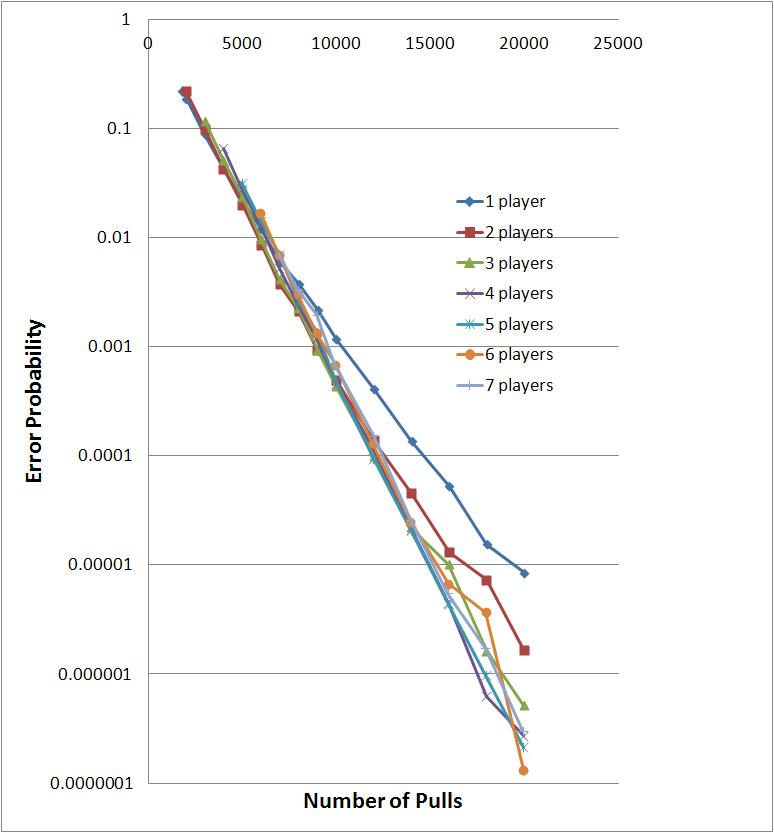
\includegraphics[scale=0.5]{figures/Error_Prob_Separate_SE_v1.jpg}
\caption{Simple SE algorithm best arm identification error probability as functions of the number of pulls for several numbers of players.}
\label{fig:Fagin1StepError}
\end{figure*}

We measure the error probability of the algorithm as a function of the total number of pulls, with 1 to 5 players. The instance set up is of a worst case scenario, which includes one ``good'' arm $P_g=0.5$ and one group of ``bad'' arms $P_b=0.4$ (total of $K=20$ arms). The results (log scaled) are depicted in Figure~\ref{fig:Fagin1StepError}.

\comment{In a distributed setting the total number of pulls are equally divided among all players, moreover, the share of each player is divided into $K$ phases. As a result, there is a minimal number of pulls $n^x$ required to allow running the game with $x$ players; namely, allowing each player to pull at least once each surviving arm per phase.}
Figure~\ref{fig:Fagin1StepError} shows that as the number of pulls increases, passing some threshold above the minimal number of pulls, running with more players exhibits lower error probability than running with a single player.

\comment{Experimenting with a different flavour of the algorithm appling a full Fagin algorithm instead of a single fagin step presents similar results, with a neglegable reduction of the error probability when running with more than one player.}

\subsection{Communication Intensive Successive Elimination}

Here we use the SE algorithm (see \ref{sec: SE algo}) with a slight modification which is dictated by the communication restrictions we apply. In particular, in each of the algorithm phase we eliminate the approximated ``worst'' arm using a restricted version of Fagin's algorithm (see \ref{sec: Fagin algo}. Accordingly, in phase A we restrict the number of index broadcasts not to exceed $L$ transmissions. It is evident that in this case errors may occur and occasionally not the ``worst'' arm is eliminated.

%\subsection{Average Number of Broadcasts}
It is easily verified that the total number of broadcasts (during both phases and assuming $L\le K$) is upper bounded by
\begin{equation}
\begin{aligned}
N_b & \le \sum_{k=1}^{\max\set{K-L+1,K-1}} 2 k L M+  
\sum_{k=K-L+2}^{K-1} 2 k (K-k+1)M\ .
\end{aligned}
\end{equation}
Evidently from the way our system is designed, the number of broadcasts is independent of the number of pulls. As a baseline for comparing communication loads a naive system where all pulls are broadcasts to all players is considered. Such a system uses $Mn$ broadcasts.

\begin{figure*}[t]
\centering
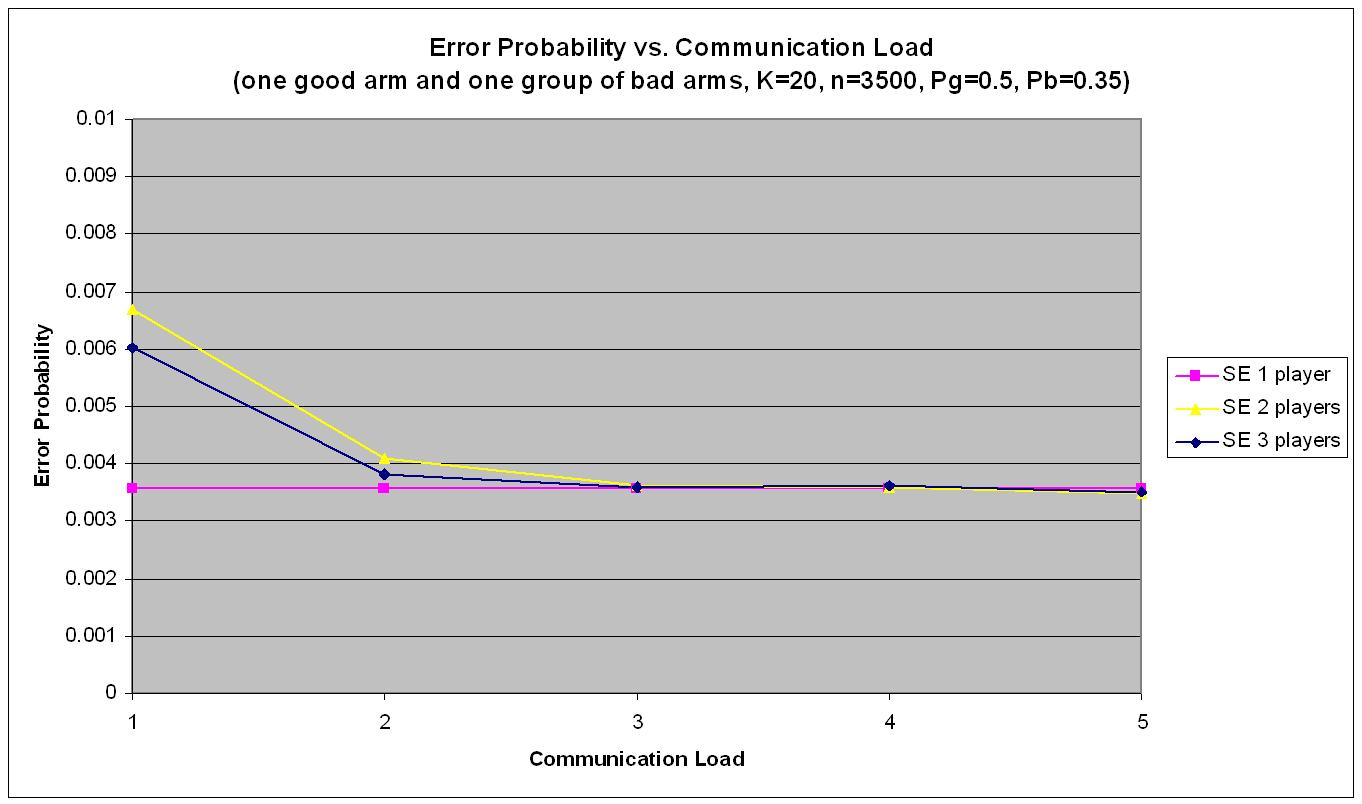
\includegraphics[scale=0.4]{figures/Error_Prob.jpg}
\caption{Communication intensive SE best arm identification error probability as functions of the communication limitation for several numbers of players.}
\label{fig: error}
\end{figure*}

\subsubsection{Error Probability Analysis}

\begin{itemize}
\item[$L_k^m$:] arms to be transmitted by player $m$ at round $k$
\item[$A_k$:] surviving arms after round $k$
\item[$B_k$:] candidates to be dismissed at the end of round $k$
\end{itemize}

\begin{itemize}
\item[$C$:] $\exists k, \exists j, |\meant{j}{n_k} - \mean{j}| > \frac{\delmean{(K+1-k)}}{\alpha}$ (where $\alpha \geq 2$) 
\item[$D$:] $\exists k, \forall j\in B_k: \alpha\delmean{j} < \delmean{(K+1-k)}$
\item[$\phi$:]$\forall k, \exists m, \forall l\in \{(K), (K-1),\ldots,(K+1-k)\}, \forall j:\alpha\delmean{j}\leq\delmean{l},  \meanp{j}{\frac{n_k}{M}}{m} > \meanp{l}{\frac{n_k}{M}}{m} $
\item[$\neg\phi$:]$\exists k,\forall m, \exists l\in \{(K), (K-1),\ldots,(K+1-k)\}, \exists j:\alpha\delmean{j}\leq\delmean{l},  \meanp{j}{\frac{n_k}{M}}{m}  \leq \meanp{l}{\frac{n_k}{M}}{m}$
\end{itemize}

\begin{eqnarray*}
D &\Rightarrow&  \neg\phi\\
\pr{e_n} &\leq& \pr{C \cup D} \leq \pr{C} + \pr{D}\\
&\leq& \pr{C} + \pr{\neg\phi}
\end{eqnarray*}

%%%%%%C
\begin{eqnarray*}
&& C: \exists k, \exists j, |\meant{j}{n_k} - \mean{j}| > \frac{\delmean{(K+1-k)}}{\alpha} \\
\pr{C} &\leq&  2\sum_{k=1}^{K-1}\sum_{j=1}^{K} \pr{\meant{j}{n_k}-\mean{j}>\frac{\delmean{(K+1-k)}}{\alpha}}\\
&\leq& 2\sum_{k=1}^{K-1}\sum_{j=1}^{K} \exp{-\frac{2n_k\delmean{(K+1-k)}^2}{\alpha^2}}\\
&\leq& 2\sum_{k=1}^{K-1}\sum_{j=1}^{K} \exp{-\frac{n-K}{\overline{log}(K)H_2}\frac{2}{\alpha^2}}\\
&\leq& 2K^2 \exp{-\frac{n-K}{\overline{log}(K)H_2}\frac{2}{\alpha^2}}\\
\end{eqnarray*}


%%%%%D=>
\begin{equation*}
\begin{aligned}
& \neg\phi: \exists k,\forall m, \exists l\in \{(K), (K-1),\ldots,(K+1-k)\}, \\
&\quad\quad \exists j:\alpha\delmean{j}\leq\delmean{l},  \meanp{j}{\frac{n_k}{M}}{m}  - \meanp{l}{\frac{n_k}{M}}{m}\leq 0\\
\pr{\neg\phi} &\leq  \sum_{k=1}^{K-1} (\sum_{l\in \{(K),\ldots,(K+1-k)\}, j: \alpha\delmean{j} \leq \delmean{l}} \pr{\meanp{j}{\frac{n_k}{M}}{m} - \meanp{l}{\frac{n_k}{M}}{m} \leq 0})^{M} \\
&\leq \sum_{k=1}^{K-1} (\sum_{l\in \{(K),\ldots,(K+1-k)\}, j: \alpha\delmean{j} \leq \delmean{l}} \exp{(-\frac{n_k}{M}{(\delmean{l}-\delmean{j})}^2)})^{M}\\
&\leq \sum_{k=1}^{K-1} (kK \exp{(-\frac{n_k}{M}\delmean{(K+1-k)}^2}(1-\frac{1}{\alpha})^2))^{M} \\
&\leq \sum_{k=1}^{K-1} (kK \exp{(-\frac{1}{M}\frac{n-K}{\overline{log}(K)H_2})(1-\frac{1}{\alpha})^2)}^{M}\\
&\leq \sum_{k=1}^{K-1} (kK)^{M} \exp{(-\frac{n-K}{\overline{log}(K)H_2})(1-\frac{1}{\alpha})^2)} \\
&\leq K^{2M+1} \exp{(-\frac{n-K}{\overline{log}(K)H_2})(1-\frac{1}{\alpha})^2)}\\
\end{aligned}
\end{equation*}

\[
\pr{e_n} \leq 2K^2 \exp{-\frac{n-K}{\overline{log}(K)H_2}\frac{2}{\alpha^2}} + K^{2M+1} \exp{(-\frac{n-K}{\overline{log}(K)H_2})(1-\frac{1}{\alpha})^2)}
\]

when $\alpha = \sqrt{2}+1$

\[
\pr{e_n} = O(K^{2M+1} \exp{(-\frac{0.34n-K}{\overline{log}(K)H_2})})
\]




\remove{
We focus on the special case where only two players are involved and a single index broadcast round is permitted ($M=2$ and $L=1$)
\begin{equation}
\begin{aligned}\label{eq:error prob}
e_n &= Pr\paren{J_n\neq i^*}= Pr\paren{A_K\neq\set{i^*}}
=Pr\paren{\bigcup_{k=1}^{K-1} i^*\notin A_{k}}\\
&\overset{(a)}{\le} \sum_{k=1}^{K-1}Pr\paren{i^*\notin A_{k}}\\
&\overset{(b)}{=}\sum_{k=1}^{K-1}Pr\paren{i^*=\argmin_{i\in B_k} \hat{X}_{i,n_k}}\\
&=\sum_{k=1}^{K-1}\left(\paren{Pr\paren{i^*=i^1_k}}^2+
2Pr\paren{i^*=i^1_k}\cdot\right.\\
&\quad\quad\quad\quad\left.\cdot Pr\paren{\hat{X}_{i^*,n_k}\le \hat{X}_{i^2_k,n_k}|i^*=i^1_k,i^*\neq i^2_k}\right)\\
&\overset{(c)}{\le}\sum_{k=1}^{K-1}Q_k\Bigg(Q_k+2\cdot\\
&Pr\paren{\left.\bigcup\begin{array}{c}
    \hat{X}^1_{i^*,n_k}\le \hat{X}^2_{i^2_k,n_k}\cap\hat{X}^2_{i^*,n_k}\le \hat{X}^1_{i^2_k,n_k}\\
    \hat{X}^1_{i^*,n_k}\ge \hat{X}^2_{i^2_k,n_k}\cap\hat{X}^2_{i^*,n_k}\le \hat{X}^1_{i^2_k,n_k}\\
    \hat{X}^1_{i^*,n_k}\le \hat{X}^2_{i^2_k,n_k}\cap\hat{X}^2_{i^*,n_k}\ge \hat{X}^1_{i^2_k,n_k}
\end{array}\right|i^*=i^1_k,i^*\neq i^2_k}\Bigg)\\
&\le \sum_{k=1}^{K-1}Q_k\paren{Q_k+6Pr\paren{\hat{X}^2_{i^*,n_k}\le \hat{X}^1_{i^2_k,n_k}|i^*=i^1_k,i^*\neq i^2_k}}
\end{aligned}
\end{equation}
where (a) is due to the union bound;\\
(b) $B_{k}\triangleq\bigcup_{m=1}^M i^m_k$ where $i^m_k=\argmin_{i\in A_k}\set{\hat{X}^m_{i,n_k}}$;\\ (c) $Q_k\triangleq Pr\paren{i^*=i^1_k}$.

Assessing the second probability expression in the last line of \eqref{eq:error prob} resists our attempt so far. We conjecture that the condition doesn't change much and that the probability is in the order of $Q_k$. 

Following the proof of \cite[Thm. 2]{Audibert-Bubeck-Munos-COLT2010}, and recalling that each player uses half of the pull budget we have
\begin{equation}\label{eq:Qk upper bound}
Q_k\le k\exp{\paren{-\frac{n-2K}{2H_2\overline{\log}\paren{K}}}}\ .
\end{equation}

Assuming our conjecture holds we have that
\begin{equation}
\begin{aligned}\label{eq:error prob final}
e_n&\le \sum_{k=1}^{K-1}7k^2Q_k^2\\
&=\frac{7}{6}K\paren{K-1}\paren{2K-1}
\exp{\paren{-\frac{n-2K}{H_2\overline{\log}\paren{K}}}}\\
&\le 3K^3 \exp{\paren{-\frac{n-2K}{H_2\overline{\log}\paren{K}}}} .
\end{aligned}
\end{equation}
Hence, the fact that two players are pulling the arms, sharing their information by a single index broadcast each, does not change the upper bound exponent rate in the number of pulls $n$. 

\noindent \textbf{Remarks}:
\begin{itemize}
    \item It is obvious that the error probability for a fixed number of players is a decreasing function of the $L$
\item Moreover, in the limit where $L=K$ the correct arm is eliminated in each SE phase and the error probabilities of the restricted and non-restricted setups coincides with that of the single player setup
\end{itemize}
}

\subsubsection{Numerical Evaluation}

In Figure \ref{fig: error} Monte-Carlo simulations of the error probability of the distributed SE algorithm are plotted as functions of the maximum number of index broadcasts $L$, for several number of players. The curves are plotted for a worst case setup which includes  one ``good'' arm and a one group of ``bad'' arms (total of $K=20$ arms).

A few observations:
\begin{itemize}
\item As expected the probability of error reduces with increasing values of $L$ and coincides with the centralized case (one player)
\item Fixing $L$, the probability of error reduces with the number of players $M>1$ (remark: we should prove it analytically)  
\end{itemize}

\section{Concluding Remarks}

We have experimented with two distributed variants of the SE algorithm. Trying to mimic the centralized setup where only one player is considered we have formulated the communication intensive SE algorithm. Numerical evaluation reveals a general trend in which the probability of error decreases when the number of broadcasts after each SE round increases. Moreover, with unlimited number of broadcasts the probability of error of the distributed setup converges to that of the centralized one.

The second approach includes separate SE algorithm by each player and a final phase where information regarding the winning arms is shared. Surprisingly, this scheme that does not mimic the centralized setup performs better when the number of pulls is above a certain threshold. 
\comment{It is conjuctured that by conducting separate SE algorithms by each player we create an interplay between two trends. Using less pulls by each player the probability that the correct arm will be selected a player is decreased. On the other hand the final phase where information regarding the winning arms is shared provides a kind of ``soft'' decision that...} 


% Figures




% ------------------------------------------------------------------------
% Acknowledgment
% ------------------------------------------------------------------------

%\section*{Acknowledgment}

% ------------------------------------------------------------------------
% Bibliography
% ------------------------------------------------------------------------
\bibliographystyle{abbrv}
\bibliography{Reference_List_Yahoo}

%------------------------------------------------------------------------
% Appendices
%------------------------------------------------------------------------

%\input{appendices}

\end{document}
